% mental note to run makeindex on final compilation

\documentclass[a5paper,draft]{memoir}

\usepackage{parskip}
\usepackage{makeidx}
\usepackage{amssymb}
\usepackage{amsmath}
\usepackage{tabu}
\usepackage{tabularx}
\usepackage{systeme}
\usepackage{graphicx}

%\graphicspath{{subdir1/}{subdir2/}{subdir3/}...{subdirn/}}
\graphicspath{{screenshots/}}

% lambda
	% http://tex.stackexchange.com/questions/290165/how-do-i-get-a-nicer-lambda
	% ref.: egreg at http://tex.stackexchange.com/a/14406/
	\usepackage{pifont}
	\makeatletter
	\newcommand\Pimathsymbol[3][\mathord]{%
		#1{\@Pimathsymbol{#2}{#3}}}
	\def\@Pimathsymbol#1#2{\mathchoice
		{\@Pim@thsymbol{#1}{#2}\tf@size}
		{\@Pim@thsymbol{#1}{#2}\tf@size}
		{\@Pim@thsymbol{#1}{#2}\sf@size}
		{\@Pim@thsymbol{#1}{#2}\ssf@size}}
	\def\@Pim@thsymbol#1#2#3{%
		\mbox{\fontsize{#3}{#3}\Pisymbol{#1}{#2}}}
	\makeatother
	% the next two lines are needed to avoid LaTeX substituting upright from another font
	\input{utxmia.fd}
	\DeclareFontShape{U}{txmia}{m}{n}{<->ssub * txmia/m/it}{}
	% you may also want
	\DeclareFontShape{U}{txmia}{bx}{n}{<->ssub * txmia/bx/it}{}
	% just in case
	%\DeclareFontShape{U}{txmia}{l}{n}{<->ssub * txmia/l/it}{}
	%\DeclareFontShape{U}{txmia}{b}{n}{<->ssub * txmia/b/it}{}
	% plus info from Alan Munn at http://tex.stackexchange.com/questions/290165/how-do-i-get-a-nicer-lambda?noredirect=1#comment702120_290165
	\newcommand{\pilambdaup}{\Pimathsymbol[\mathord]{txmia}{21}}

% linear algebra
	% http://tex.stackexchange.com/questions/2233/whats-the-best-way-make-an-augmented-coefficient-matrix
	\newenvironment{amatrix}[1]{%
		\left(\hspace{0.15cm}\begin{array}{@{}*{#1}{c}|c@{}}
		}{%
	\end{array}\hspace{0.15cm}\right)
	}
	
	\def\VR{\kern-\arraycolsep\strut\vrule &\kern-\arraycolsep}
	\def\vr{\kern-\arraycolsep & \kern-\arraycolsep}

\pretitle{\begin{center}\Huge\bfseries}
	\title{A Comprehensive Guide to the CASIO fx-9860GIIs}
	\posttitle{\par\vskip1em{\normalfont\normalsize\scshape The better graphing calculator for the H2 Maths Syllabus \\ \vspace{1cm} Quick Reference Math included\par\vfill}\end{center}}
\author{Sun Yudong, Li Yicheng \\ 15S6G \\ Hwa Chong Institution (College Section)}
\predate{\vfill\begin{center}\large}

\def\code#1{\texttt{#1}}
\def\note#1{\textbf{\textit{Note:}} #1}
\def\tip#1{\textbf{\textit{Tip:}} #1}

\setlength{\parindent}{0pt}
\setlength{\parskip}{1ex plus 0.5ex minus 0.2ex}

%\setcounter{tocdepth}{2} % which level the sectioning commands are printed in the ToC
%\setcounter{secnumdepth}{4} %up to what level the sectioning titles are numbered\makeatletter
\setsecnumdepth{subsection}

\newcommand{\addtoindex}[1]{#1\index{#1}}

\begin{document}

\begin{titlingpage}
	\maketitle
\end{titlingpage}

\frontmatter

\tableofcontents

\chapter{Preface}
This guide is provided as-is and was compiled by a bunch of students in 2016. We tried our best to be mathematically and technically accurate. But software versions (Ver 2.04 now) do change, and this guide may not be valid indefinitely. However, the source of this file is publically available on GitHub. Feel free to contact us.

If there are anything you want to do, but you can't seem to know how to, try Google, or RTFM. Otherwise, just experiment a bit. The CASIO interface should be intuitive enough.

Do note that some notes inside this guide were taken from the H2 Mathematics notes provided by the Hwa Chong Institution (College Section) Math Department. 

\vspace{0.7cm}

\begin{tabular}{l l}
	Sun Yudong: & sunjerry019 [at] gmail [dot] com \\
	Li Yicheng: & liyicheng340 [at] gmail [dot] com 
\end{tabular}


\mainmatter
\chapter{The Basics}
Every command you will ever need is organized neatly in the \code{[OPTN]} button on your graphing calculator (GC).

Unfortunately there are some areas where the CASIO calculator isn't very intuitive and we need some documentation.

\tip{You can just press the button that corresponds to the number/letter at the bottom right of the icons in the menu:}

\begin{figure}[h]
	\centering
	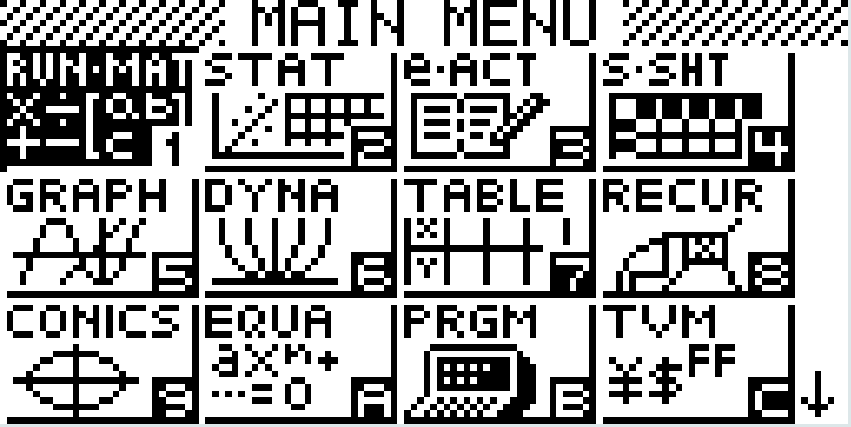
\includegraphics[width=0.5\textwidth]{mainmenu}
\end{figure}

\section{Graphing} \label{graphing}
To graph a function, go to \code{GRAPH} in the main menu. Enter the functions into \code{Y1} onwards. Press \code{DRAW} (\code{F6}) or \code{[EXE]} to graph. Most of these are pretty intuitive, just some things you should take note:
\begin{itemize}
	\item The \code{Y} and \code{X}, etc. at the bottom of the screen is for entering the functions \code{Y1, Y2, \dots} and \code{X1, X2, \dots}. For the variable $x$, use the \code{[X,$\theta$,T]} button instead
	\item To restrict the domain of the function, type:
	\begin{center}
		\code{Y1 = $f(x)$,[start,end]}
	\end{center}
\end{itemize}

After pressing \code{DRAW} (\code{F6} or \code{[EXE]}), you can press \code{[AC/on]} to break the plotting script.

To solve for anything, use \code{[G-Solv]} (\code{F5}).

\subsection{Plotting a table from function} \label{plottable}
Plot using function


\section{Solving for the roots of a polynomial}
There are mainly 2 ways to solve for the roots of a polynomial using the GC:
\begin{itemize}
	\item Using the \code{EQUA > Poly} (\code{F2}) app
	\item Plot a graph and solve for roots
\end{itemize}

The \code{EQUA > Poly} is quite intuitive, and similar to the standard issue CASIO fx-95SG scientific calculator, so we will just note some limitations/features of this GC:
\begin{itemize}
	\item The polynomial solver only accepts real coefficients
	\item You can change the \code{Set Up > Complex Mode} setting to \code{$a+bi$} for imaginary roots (but not imaginary coefficients)
\end{itemize}

To plot a graph, you go to \code{Graph}. Refer to Section \ref{graphing} (Graphing) for more information.

\section{Solving a 1-variable Equation}
There are mainly 2 ways to solve a 1-variable equation (e.g. $e^x + 5x = 1$) using the GC:
\begin{itemize}
	\item Using the \code{EQUA > Solver} (\code{F3}) app
	\item Using \code{Solve} or \code{SolveN}
	\item Plotting a graph
	\begin{itemize}
		\item Move everything to one side and solve for root
		\item Solve for the intersections of 2 or more graphs
	\end{itemize}
\end{itemize}

\subsection{Solving using \code{EQUA > Solver}}
To use the built-in equation solver:
\begin{enumerate}
	\item Go to \code{EQUA > Solver} (\code{F3})
	\item Enter the equation you would like to solve under \code{Eq}. Remember to put the = sign.
	\begin{itemize}
		\item Alternatively, you can use \code{RCL} (\code{F1}) to recall functions entered into \code{GRAPH} or \code{TABLE}
	\end{itemize}
	\item Press \code{[EXE]} and put your initial guess under \code{X}. An example can be as such:
	\begin{center}
		\code{
			\begin{tabular}{|r|l|}
				\hline
				X 		& 0 \\
				\hline
				Lower 	& -9E+99 \\
				\hline
				Upper	& 9E+99 \\
				\hline
			\end{tabular}
		}
	\end{center}
	\item Press \code{Solv} (\code{F6})	
\end{enumerate}

\note{}The initial guess isn't very important for equations with unique solutions. However, if the equation has multiple solutions, it will give the answer closer to the original guess.

For example, given the equation $(x-1)(x-3)=0$, entering the following will give the corresponding answers:
\begin{center}
	\renewcommand{\arraystretch}{1.2}
	\begin{tabular}{|c|c|}
		\hline
		$X$ 	& Answer \\
		\hline
		0		& 1 \\
		\hline
		1.5 	& 1 \\
		\hline
		2		& 1 \\
		\hline
		2.5		& 3 \\
		\hline
		4		& 3 \\
		\hline
	\end{tabular}
\end{center}

After solving the equation, you can always access the value again by going to \code{RUN$\cdot$MAT} and typing \code{X}.

\subsection{Solving using \code{Solve} or \code{SolveN}}
Alternatively, you can use the \code{Solve} or \code{SolveN} functions to obtain the solution. They can be found under \code{[OPTN] > CALC}(\code{F4}).

Their usage is as follows, as far as we have discovered:
\begin{center}
	\code{Solve(<equation>,<initial guess>)} \\
	\code{SolveN(<equation>)}
\end{center}

\section{Solving a Multi-variable Linear System}
There are 3 types of linear systems, namely systems with:
\begin{itemize}
	\item No solution
	\item 1 unique solution
	\item Infinitely many solutions
\end{itemize}

To solve a multi-variable system of linear equations using your GC, there are 2 main ways:
\begin{enumerate}
	\item Using the \code{EQUA > Siml} (\code{F1}) app
	\item Using matrices
\end{enumerate}

\subsection{Using the \code{EQUA > Siml} app}
While you can use matrices to solve any kind of linear system, you can use the \code{EQUA > Siml} app \textit{\textbf{only if the linear system has a unique solution}}.

\note{Should you try to use the \code{EQUA > Siml} app to solve for a linear system with no solution, or infinitely many solutions, the calculator would just throw a \code{Ma Error} at you while you stare, bemused, wondering why the calculator is so bad to you.}

Anyhow, the app is intuitive enough, so I shall skip it.

\subsection{Using Matrices}

To solve a linear system the matrix way, let's first consider the following linear system:
\begin{center}
	\syslineskipcoeff{1.2}
	\systeme{
		\hspace{0.2cm} x+y+2z=9,
		\hspace{0.2cm} 2x+4y-3z=1,
		\hspace{0.2cm} 3x+6y-5z=0
	}
\end{center}

By taking the coefficients of the variables $x$, $y$ and $z$, we can form the following augmented matrix:
\[
	\begin{amatrix}{3}
		1 & 1 & 2  & 9 \\  
		2 & 4 & -3 & 1 \\
		3 & 6 & -5 & 0
	\end{amatrix}
\]

To solve for $x$, $y$ and $z$:\footnote{ Fn Keys have been left out to save space.}
\begin{enumerate}
	\item Go to \code{RUN$\cdot$MAT > $\triangleright$MAT}
	\item Select \code{Mat A} and enter the dimensions
	\begin{itemize}
		\item $m$ is the number of rows, in this case 3
		\item $n$ is the number of columns, in this case 4
	\end{itemize}
	\item Enter the augmented matrix above accordingly, putting the augmented column into the 4th column:
	\begin{equation*}
		\left[
			\begin{array}{cccc}
			1 & 1 & 2  & 9 \\  
			2 & 4 & -3 & 1 \\
			3 & 6 & -5 & 0
			\end{array}
		\right]
	\end{equation*}
	\item Press \code{[EXIT]} then \code{[EXIT]} to go back to the main \code{RUN$\cdot$MAT} screen
	\item Go to \code{[OPTN] > MAT > $\triangleright$ > Rref}
	\item Then \code{ $\triangleright \times 3$ > Mat}, then \code{[ALPHA] + A}, giving the following:
	\begin{center}
		\code{Rref Mat A}
	\end{center}
	\item Press \code{[EXE]}, and then you should be able to get the following matrix:
	\begin{equation*}
		\left[
			\begin{array}{cccc}
			1 & 0 & 0 & 1 \\  
			0 & 1 & 0 & 2 \\
			0 & 0 & 1 & 3
			\end{array}
		\right]
	\end{equation*}
\end{enumerate}

This can then be rewritten as an augmented matrix:
\begin{equation*}
\bordermatrix{  & x & y & z & \vr ~ \cr
			  ~ & 1 & 0 & 0 & \VR 1 \cr
			  ~ & 0 & 1 & 0 & \VR 2 \cr
			  ~ & 0 & 0 & 1 & \VR 3 }
\end{equation*}

which can then be rewritten as:
\begin{center}
	\syslineskipcoeff{1.2}
	\systeme{
		\hspace{0.2cm} x=1,
		\hspace{0.2cm} y=2,
		\hspace{0.2cm} z=3
	}
\end{center}

Notice that the left side of the final augmented matrix is the identity matrix. This is what you would typically see for a linear system with a unique solution.

This same procedure can be used to find the solutions of any linear system with any number of variables.

The following are possible matrices you can obtain after the \code{Rref} command for the other types of linear systems:

\begin{itemize}
	\item \textbf{No solution}
	\begin{equation*}
		\begin{tabu}{ccc}
			\begin{amatrix}{3}
			1 & 0 & 2 & 2 \\  
			0 & 1 & 3 & 3 \\
			0 & 0 & 0 & 1
			\end{amatrix} & \rightarrow & \syslineskipcoeff{1.2}
			\systeme{
				\hspace{0.2cm} x=2-2t,
				\hspace{0.2cm} y=3-3t,
				\hspace{0.2cm} 0z=1
			}\\
		\end{tabu}
	\end{equation*}
	where $t \in \mathbb{R}$
	
	Since $0=1$ is not possible, the above linear system is inconsistent and has no solutions.
	\item \textbf{Infinitely many solutions}
	\begin{equation*}
		\begin{tabu}{ccc}
			\begin{amatrix}{3}
			1 & 0 & 2 & 2 \\  
			0 & 1 & 3 & 3 \\
			0 & 0 & 0 & 0
			\end{amatrix} & \rightarrow & \syslineskipcoeff{1.2}
			\systeme{
				\hspace{0.2cm} x=2-2t,
				\hspace{0.2cm} y=3-3t,
				\hspace{0.2cm} z=t
			}\\
		\end{tabu}
	\end{equation*}
	where $t \in \mathbb{R}$
	
	In this case, the answer is obtained easily through back-substitution. Rewriting the augmented matrix, we observe that:
	\begin{center}
		\syslineskipcoeff{1.2}
		\systeme{
			\hspace{0.2cm} x+2z=2,
			\hspace{0.2cm} y+3z=3
		}
	\end{center}
	
	By letting $z$ be a parameter $t$ ($t \in \mathbb{R}$), we observe that:
	\begin{equation*}
	\begin{tabu}{ccc}
		\syslineskipcoeff{1.2}
		\systeme{
			\hspace{0.2cm} x+2t=2,
			\hspace{0.2cm} y+3t=3,
			\hspace{0.2cm} z=t
		} & \rightarrow & \syslineskipcoeff{1.2}
			\systeme{
				\hspace{0.2cm} x=2-2t,
				\hspace{0.2cm} y=3-3t,
				\hspace{0.2cm} z=t
			}\\
		\end{tabu}
	\end{equation*}
	
	Thus obtaining the general solution. 
\end{itemize}

You will find this useful for both "System of Linear Equations" and "Vectors" (See Chapter \ref{vectors}). 

For a more in-depth understanding of what is going on here, you may wish to refer to Section \ref{solvLinSys}.

\section{Taking Integrals}
\subsection{Definite Integrals}
Your calculator can be used to solve definite integrals.

One way is to find the area under the graph after plotting the equation.

\begin{enumerate}
	\item Plot the graph following the instructions from Section \ref{graphing}.
	\item Press \code{G-Solv} (\code{F5}), followed by $\triangleright$ (\code{F6}) and \code{$\int$dx} (\code{F3}).
	\item A cursor on the curve will now appear on the graph, along with $x$ and $y$ values. Move the cursor to the lower bound of the definite integral you're trying to find, and press \code{EXE}, followed by the upper bound, and press \code{EXE} again.
	\item The area under the graph should now be shaded and the value of the area is displayed as \code{$\int$dx}.
\end{enumerate}

This method is great if you already have the graph plotted and want to find the integral quickly without entering the equation again. If you do not need to plot the graph and simply want to find the definite integral directly, you may find the integration function in the \code{RUN$\cdot$MAT} app more useful.

\begin{enumerate}
	\item From the main menu, enter the \code{RUN$\cdot$MAT} app (\code{1}).
	\item Press the \code{OPTN} button and select the \code{CALC} option (\code{F4}).
	\item Under the \code{CALC} submenu, choose the \code{$\int$dx} option (\code{F4}).
	\item Enter the equation as per standard Mathematical notation. 
	
	\note{You should change the variable to be integrated from whatever letter it was originally to $x$ since the calculator forces the integral to be integrated with respect to $x$ as can be seen by the $dx$ at the back.}
\end{enumerate}

\subsection{Indefinite Integrals}
SEAB bans all calculators capable of direct symbolic integration and differentiation. In other words, you cannot enter $3x^2$ into your graphing calculator and get $x^3$ or vice versa. To be fair, this feature was never in the international version of the Casio anyway.

Thankfully, even in the Singaporean version of the Casio, you can plot the graph of the integral visually.

For example, we will try to plot the integral of $2x$. Assuming that your GC is working properly and the Laws of Mathematics have not changed in drastic ways, the graph should be identical to that of $x^2$.

\begin{enumerate}
	\item From the main menu, enter the \code{GRAPH} app (\code{5}).
	\item Under \code{Y1}, enter the function $2x$.
	\item Move to \code{Y2}. Enter the following function:
	\begin{equation*}
	\code{Y2}=\int_{0}^{x} \code{Y}1 \, dx
	\end{equation*}
	\note{\code{Y2} will take a significant amount of time to plot (around 5-10 seconds). It is recommended that you deselect \code{Y1} by pressing \code{SEL} (\code{F1}) to prevent \code{Y1} from being plotted, saving a couple of seconds.}
	\item Press \code{DRAW} (\code{F6}). A parabola that identical to $y=x^2$ should be yield. You can plot $y=x^2$ on top of the integral to confirm.
\end{enumerate}

While this function is unable to give you the equation of the integral directly, you can use double check your integrals using this method. Plotting the integral using this method can also be useful if you have to find multiple definite integrals (using the trace function in the graph page).

\chapter{Vectors} \label{vectors}

\chapter{Statistics}
One major use of a graphing calculator is for use in statistics. In the following chapters, we will outline the methods with which we can use our GC. Calculator functions in this section can generally be found under \code{[OPTN] > [STAT]}. Permutation and Combinations will not be covered. Calculated variables can be found under \code{[VARS] > [STAT]}

In this chapter, all random variables are represented by capital letters (usually $X$ or $Y$). Small letters are reserved to represent values (e.g. $x$).

\note{However, please do not use $Z$, as it is reserved for the standard normal distribution.}

\section{Discrete Random Variable}
A discrete (countable) random variable $X \in \mathbb{Z}^*$ has expectation (or expected value or mean) $\mu$
\begin{equation}
	\mathrm{E}(X)=\mu=\sum_{\mathrm{all}~x}^{}x\mathrm{P}(X=x)
\end{equation}
(You can think of this as the weighted sum of all the possibilities for $X$)

and variance $\sigma^2=\mathrm{stddev}^2$
\begin{equation}
	\mathrm{Var}(X)=\sigma^2=\mathrm{E}(X-\mu)^2=\mathrm{E}(X^2)-\mu^2
\end{equation}
\note{The above does not apply to continuous random variables.}

The function that gives the probability that a discrete random variable is exactly equal to some value is called the \textit{Probability Mass Function} (PMF). However, we will write PDF throughout this section instead, so as to be in-line with the curriculum/ calculator functions.

\subsection{Using Data}
If given a set of histogram data (i.e. categories and its corresponding frequencies), one can calculate statistical properties of it.

For example, given the following data:
$$
\setlength\tabulinesep{2mm}
\begin{tabu}{ |c|c|c|c|c| }
	\hline
	x & 0 & 1 & 2 & 3 \\
	\hline 
	\mathrm{P}(X=x)  & \frac{1}{8}  & \frac{3}{8}  & \frac{3}{8} &\frac{1}{8}  \\
	\hline
\end{tabu}
$$

You can do 1-Variable Statistical calculations by:
\begin{enumerate}
	\item Go into \code{STAT} and then enter the X-values into \code{List 1} and its frequency into \code{List 2}
	\item Go to \code{CALC > SET} and adjust the settings accordingly for 1-Var (\code{XList:List1, Freq:List2})
	\item \code{[EXIT]} and then choose \code{1VAR}
\end{enumerate}

If you want to further manipulate these calculated values (such as squaring $\sigma$ to find variance), you can go to \code{RUN$\cdot$MAT} and then \code{[VARS] > [STAT] > [X]} to finding the value(s) you wanted.

Refer to Section \ref{plotstat} (Plotting Statistics/ Visualization) for plotting statistical data.

\subsection{Binomial Distribution} \label{binom}
A binomial random variable $X$ has the following characteristics:
\begin{enumerate}
	\item The experiment consists of $n$ repeated independent trials
	\item Each trial only has 2 outcomes: "success" or "failure"
	\item The probability of a 'success' $p$ is constant in each trial
\end{enumerate}

% The probability distribution of $X$ is called the \textit{binomial distribution}, and 
The probability $\textrm{P}(X = x)$ of obtaining $x$ successes in $n$ trials is given by:

\begin{equation}
	\mathrm{P}(X=x) = {n \choose x} p^x(1-p)^{n-x},~x \in \mathbb{Z}^*
\end{equation}

and has $\mathrm{E}(X) = np$ and $\mathrm{Var}(X)=np(1-p)$.

We write $X \sim \mathrm{B}(n, p)$.

\note{the probability is only non-zero when $0 \leq x \leq n$ (i.e. there is an upper bound).}

\subsubsection{Binomial PDF}

To obtain the probability $\textrm{P}(X = x)$, we can either use the formula, or use the in-built \code{\addtoindex{BinomialPD}} function:
\begin{center}
	\code{BinomialPD(X,$n$,$p$)}
\end{center}

Alternatively, we can use the \code{STAT} app to obtain the probability:
\begin{enumerate}
	\item Go into \code{STAT} (\code{2} in the menu)
	\item Press \code{DIST}(\code{F5})\code{ > BINM}(\code{F5})\code{ > Bpd}(\code{F1})
	\item Set the following:
	\begin{center}
		\setlength{\tabcolsep}{10pt}
		\renewcommand{\arraystretch}{1.1}
		\begin{tabular}{|l|l|}
			\hline
			Data		& Variable \\
			\hline
			$x$			& X \\
			\hline
			Numtrial	& $n$ \\
			\hline
			$p$			& $p$ \\
			\hline
			Save Res	& \code{None} \\
			\hline
		\end{tabular}
	\end{center}
	\item Press \code{[EXE]} or scroll to \code{Execute} and press \code{CALC}(\code{F1})
	\item You can do further manipulation of the value obtained by:
	\begin{enumerate}
		\item Going to \code{RUN$\cdot$MAT}
		\item Go to \code{[VARS] > STAT}(\code{F3})\code{ > RESLT}(\code{F6})\code{ > DIST}(\code{F3})
		\item There you can find the $p$ value by pressing $p$ (\code{F1}) and then \code{[EXE]}
	\end{enumerate} 
\end{enumerate}

\subsubsection{Binomial CDF}

To obtain the probability $\textrm{P}(X \leq x)$ (\textit{cumulative distribution function} of $x$), we can use the in-built \code{\addtoindex{BinomialCD}} function:

\begin{center}
	\code{BinomialCD(X,$n$,$p$)}
\end{center}

Alternatively, following instructions in the previous section (Section \ref{binom} $\Rightarrow$ Binomial PDF), and choosing \code{Bcd} instead. 

As a general rule of thumb:
\begin{center}
	\setlength{\tabcolsep}{10pt}
	\renewcommand{\arraystretch}{1.1}
	\begin{tabular}{|c|c|}
		\hline
		Answer in:		& Use: \\
		\hline
		$\mathbb{Z}$	& Table \\
		\hline
		$\mathbb{R}$	& Graph \\
		\hline
	\end{tabular}
\end{center}

Refer to Section \ref{plottable} for plotting results from a table, which might be useful for plotting the PDF/CDF of a binomial distribution, since $\mathrm{P}(X=x)$ is undefined when $x \notin \mathbb{Z}^*$

\subsection{Poisson Distribution} \label{poisson}
A random variable that follows a Poisson distribution has the following characteristics:
\begin{itemize}
	\item Events occur randomly in a fixed interval and independently of one another.
	\item The mean rate of occurrence of the event is \textbf{constant} in the given interval.
	\item The probability of more than 1 event occuring within a short interval is \textbf{negligible}. 
\end{itemize}

The probability $\textrm{P}(X = x)$ of obtaining $x$ successes in a fixed interval is given by:
\begin{equation}
	\textrm{P}(X=x)=e^{-\pilambdaup}\frac{\pilambdaup^x}{x!},~x \in \mathbb{Z}^*
\end{equation}

We write $X \sim \textrm{Po}(\pilambdaup)$, where $\pilambdaup$ is the mean number of occurrence of the event in that fixed interval. 

This random variable $X$ has $\mathrm{E}(X)=\mathrm{Var}(X)=\pilambdaup$.

\note{}
\begin{itemize}
	\item $X$ ranges over an infinite number of integer values (i.e. there is no upper bound)
	\item $\pilambdaup \propto t$, where $t$ is the length of the interval
\end{itemize}

\note{}
\begin{center}
	\setlength{\tabcolsep}{10pt}
	\renewcommand{\arraystretch}{1.1}
	\begin{tabular}{|c|c|}
		\hline 
		$\pilambdaup \in \mathbb{Z}$					& 2 modes\\
		\hline
		$\pilambdaup \in \mathbb{R} \notin \mathbb{Z}$	& 1 mode\\
		\hline
	\end{tabular}
\end{center}

\subsubsection{Poisson PDF}
To obtain the probability $\textrm{P}(X = x)$, we can either use the formula, or use the in-built \code{\addtoindex{PoissonPD}} function:
\begin{center}
	\code{PoissonPD(x,$\pilambdaup$)}
\end{center}

Alternatively, we can use the \code{STAT} app to obtain the probability:
\begin{enumerate}
	\item Go into \code{STAT} (\code{2} in the menu)
	\item Press \code{DIST}(\code{F5})\code{ > POISN}(\code{$\triangleright$ F1})\code{ > Ppd}(\code{F1})
	\item Set the following:
	\begin{center}
		\setlength{\tabcolsep}{10pt}
		\renewcommand{\arraystretch}{1.2}
		\begin{tabular}{|l|l|}
			\hline
			Data		& Variable \\
			\hline
			$x$			& X \\
			\hline
			$\mu$		& $\pilambdaup$ \\
			\hline
			Save Res	& \code{None} \\
			\hline
		\end{tabular}
	\end{center}
	\item Press \code{[EXE]} or scroll to \code{Execute} and press \code{CALC}(\code{F1})
	\item You can do further manipulation of the value obtained by:
	\begin{enumerate}
		\item Going to \code{RUN$\cdot$MAT}
		\item Go to \code{[VARS] > STAT}(\code{F3})\code{ > RESLT}(\code{F6})\code{ > DIST}(\code{F3})
		\item There you can find the $p$ value by pressing $p$ (\code{F1}) and then \code{[EXE]}
	\end{enumerate} 
\end{enumerate}

\subsubsection{Poisson CDF}
The cumulative probability $\textrm{P}(X \leq x)$ can be calculated by using the in-built \code{\addtoindex{PoissonCD}} function:
\begin{center}
	\code{PoissonCD(x,$\pilambdaup$)}
\end{center}

Alternatively, following instructions in the previous section (Section \ref{poisson} $\Rightarrow$ Poisson PDF), and choosing \code{Pcd} instead. 

\subsubsection{Additive Property of Poisson Random Variable}
If $X \sim \textrm{Po}(\pilambdaup)$ and $Y \sim \textrm{Po}(\mu)$, where $X$ and $Y$ are \textbf{independent}, then:
\begin{equation}
	X+Y \sim \textrm{Po}(\pilambdaup + \mu)
\end{equation}

\section{Continuous Random Variable}
The probability for a continuous variable $X$ to fall within a particular region $[a,b]$ is given by:
\begin{equation}
	\mathrm{P}(a \leq X \leq b) = \int_{a}^{b} f(x)
\end{equation}
where $f(x)$ is the \textit{probability density function} (PDF) of X.

In particular,
\[
\int_{-\infty}^{\infty}f(x) = 1
\]

Moreover, 
\begin{align*}
	\mathrm{P}(a \leq X \leq b) &= \mathrm{P}(a \leq X < b)\\
	&= \mathrm{P}(a < X \leq b) \\
	&= \mathrm{P}(a < X < b)
\end{align*}

\subsection{Normal Distribution}
A (continuous) random variable $X\in \mathbb{R}$ that follows a normal distribution with mean $\mu$ and standard deviation $\sigma$ has a \textit{probability density function} (PDF) given by:

\begin{equation}
	f(x)=\frac{1}{\sigma\sqrt{2\pi}} \cdot e^{\frac{-(x-\mu)^2}{2\sigma^2}}
\end{equation}

We write $X \sim \mathrm{N} (\mu,\sigma^2)$

\note{$Z$ is reserved to represent the standard normal distribution. Do not use it to represent your variables (that do not follow standard normal distribution).}

\subsubsection{Normal Distribution PDF}
There are one of 2 ways to plot a graph of the normal distribution PDF:

\begin{itemize}
	\item Plot the actual equation
	\item Use the in-built \code{NormPD} function
\end{itemize}

However, it must be noted that the \code{NormPD} plots slower than using the actual equation. Using \code{G-Solv} is also slower.

The usage of \code{\addtoindex{NormPD}} is 
\begin{center}
	\code{NormPD(X,$\sigma$,$\mu$)}
\end{center}

\note{You should not use this command to calculate the probability of a certain random variable $\textrm{P}(X = x)$ where $x \in \mathbb{R}$. This is because for a continuous random variable, this does not make sense. It should always be a range. (i.e. use the CDF in the next section)}

\subsubsection{Normal Distribution CDF}
CDF stands for \textit{Cumulative Distribution Function}. This can be calculated by taking the integral of the normal PDF from $-\infty$ to $x$. One can take integral by plotting the graph out (refer to previous section), and then \code{G-Solv > $\int$dx}.

Alternatively, you can use the built-in \code{\addtoindex{NormCD}}:
\begin{center}
	\code{NormCD([Lower],[Upper],$\sigma$,$\mu$)}
\end{center}

To plot the Normal Distribution CDF, you can use:
\begin{center}
	\code{Y = NormCD(-1E99,X,$\sigma$,$\mu$)}
\end{center}

\note{\code{-1E99} is to simulate $-\infty$.}

Alternatively, we can use the \code{STAT} app to obtain the probability:
\begin{enumerate}
	\item Go into \code{STAT} (\code{2} in the menu)
	\item Press \code{DIST}(\code{F5})\code{ > NORM}(\code{F1})\code{ > Ncd}(\code{F1})
	\item Set the following:
	\begin{center}
		\setlength{\tabcolsep}{10pt}
		\renewcommand{\arraystretch}{1.2}
		\begin{tabular}{|l|l|}
			\hline
			Data		& Variable \\
			\hline
			Lower		& \textit{Lower} \\
			\hline
			Upper		& \textit{Upper} \\
			\hline
			$\sigma$	& $\sigma$ \\
			\hline
			$\mu$		& $\mu$ \\
			\hline
			Save Res	& \code{None} \\
			\hline
		\end{tabular}
	\end{center}
	\item Press \code{[EXE]} or scroll to \code{Execute} and press \code{CALC}(\code{F1})
	\item You can do further manipulation of the value obtained by:
	\begin{enumerate}
		\item Going to \code{RUN$\cdot$MAT}
		\item Go to \code{[VARS] > STAT}(\code{F3})\code{ > RESLT}(\code{F6})\code{ > DIST}(\code{F3})
		\item There you can find the $p$ value by pressing $p$ (\code{F1}) and then \code{[EXE]}
	\end{enumerate} 
\end{enumerate}
\note{You cannot use this method for plotting}

\subsubsection{Finding the value given the probability}
One sometimes need to find $a$ given $\textrm{P}(X < a) = b$ where $a,b \in \mathbb{R}$ and $b$ is the probability of $X$ being less than $a$. 

To do this, we need the \code{\addtoindex{InvNormCD}} function built into the calculator. The usage of \code{InvNormCD} is as follows:
\begin{center}
	\code{InvNormCD($b$,$\sigma$,$\mu$)}
\end{center}

This will give you back $a$.

\section{Use for Experimental Data/SPA}
The calculator can be used to determine the equation of a best fit line/parabola etc. from a set of data from experiments. From the main menu, enter the \code{S-SHT} app (\code{4}). 

In the app, simply enter each set of data into each row. Enter the data on the same axis under the same column.

For example, consider the following experimental data for an experiment involving electrical current ($I$) and potential difference ($V$): 

\begin{center}
	\setlength{\tabcolsep}{10pt}
	\renewcommand{\arraystretch}{1.2}
	\begin{tabular}{|c|c|}
		\hline
		\textbf{V/V}	& \textbf{I/A} \\
		\hline
		0.7148			& 0.0588 \\
		\hline
		0.7372			& 0.0633 \\
		\hline
		0.7780			& 0.0752 \\
		\hline
		1.058			& 0.143 \\
		\hline
		1.200			& 0.170 \\
		\hline
		1.340			& 0.210 \\
		\hline
	\end{tabular}
\end{center}

\pagebreak
Enter this set of data into the GC as follows:

\begin{center}
	\setlength{\tabcolsep}{10pt}
	\renewcommand{\arraystretch}{1.2}
	\begin{tabular}{|r|c|c|}
		\hline
		{\tiny SHEET}& \textbf{A}	& \textbf{B} \\
		\hline
		\textbf{1}	& 0.7148		& 0.0588 \\
		\hline
		\textbf{2}	& 0.7372		& 0.0633 \\
		\hline
		\textbf{3}	& 0.7780		& 0.0752 \\
		\hline
		\textbf{4}	& 1.058			& 0.143 \\
		\hline
		\textbf{5}	& 1.200			& 0.170 \\
		\hline
		\textbf{6}	& 1.340			& 0.210 \\
		\hline
	\end{tabular}
\end{center}

To plot the points onto a graph, first press the right arrow key ($\triangleright$, \code{F6}) and select the \code{GRPH} option (\code{F1}).

Once in the \code{GRPH} menu, we will first configure the graph options. 
\begin{enumerate}
	\item Press \code{SET} (\code{F6}) and ensure that \code{StatGraph1} is shown on the first line and the \code{Graph Type} is \code{Scatter}.
	\item Move to \code{XCellRange} and enter \code{B1:B6}. This means that the values from cells \code{B1} to \code{B6} inclusive are that for the horizontal $x$-axis.
	\item Move to \code{YCellRange} and enter \code{A1:A6}.
	\item Finally, ensure that the \code{Frequency} option is \code{1}.
	\begin{itemize}
		\item You may select any \code{Mark Type} that suits your personal preferences.
	\end{itemize}
	\item Press \code{EXIT} to leave the configuration menu and return to the spreadsheet.
\end{enumerate}

Now, press \code{GPH1} (\code{F1}). A graph with markings corresponding to the points on the spreadsheet should be yield.

You calculator can find the equation of a best fit line or curve. In this case, the data is expected to be linearly related (and it is linearly related).

\begin{enumerate}
	\item Press \code{CALC} (\code{F1}).
	\item There are now a number of options corresponding to different types of graphs and relationships such as $x^2$, $\ln$, and $e^x$. In this case, our data is linear, so select \code{X} (\code{F2}).
	\item Select $\code{ax+b}$ (\code{F1}).
	\item A table with various values is yield. The value $a$ corresponds to the gradient, and $b$ is the $y$-intercept. $r^2$ represents how closely the data fit to the line, with the value of $1$ corresponding to a perfect, ideal fit.
	\item To view the graph visually, select \code{DRAW} (\code{F6}). To generate $y$-values using the equation, select \code{COPY} (\code{F5}), and select one of the \code{Y1}/\code{Y2\dots} to copy to.
\end{enumerate}

\note{You will need to add an $\times$ between the gradient and the $x$, or it will cause the function to error out.}

The linear regression result can also be obtained using the concept of best approximations, covered in Section \ref{bestapprox} under Linear Algebra.

\subsection{Plotting Statistics/Visualization} \label{plotstat}


\chapter{Linear Algebra}
Some of you might find yourself doing linear algebra, and needing to do matrix manipulations. In this chapter, I will outline some basic concepts covered in MA1101R (NUS H3 Course), and how you can use your GC to find the answer.

You may find certain concepts here useful for H2 Mathematics as well, especially in terms of matrix manipulations. I suggest you read this chapter as a complement of Chapter \ref{vectors} (Vectors). 

\section{Storing Matrices}
accessing individual matrix elements

\section{Solving Linear Systems} \label{solvLinSys}
introduce augemented matrix
how to augment if 2

\subsection{Elementary Row Operations and Row-Echelon Forms}
row equiv

\section{Best Approximations} \label{bestapprox}

\printindex


\end{document}